
\begin{frame}{conclusion}{impact}
    \begin{itemize}
        \item \textbf{society \& culture}
            \begin{itemize}
                \item value of music/art, value of human origin
                \item musical bias, increasing homogeneity
            \end{itemize}
        \item \textbf{science} 
            \begin{itemize}
                \item measuring progress
            \end{itemize}
        \item \textbf{economy}
            \begin{itemize}
                \item livelihoods/workforce
                \item new business models
            \end{itemize}
        \item \textbf{environment}
            \begin{itemize}
                \item energy, local impact
            \end{itemize}
        \item \textbf{regulatory \& legal}
                \begin{itemize}
                    \item fair use terms
                    \item monopolies
                    \item labeling of ai-created content
                    \item accountability and liability
                \end{itemize}
    \end{itemize}
\end{frame}

\begin{frame}{conclusion}{conclusion}
    \vspace{-7mm}
    \begin{columns}
    \column{.65\linewidth}
        \begin{itemize}
             \item   \textbf{many opportunities}
                \begin{itemize}
                    \item increased efficiency in content production
                    \item new tech will always be used in unforeseen creative ways
                    \item accessibility increases dramatically
                \end{itemize}
            \smallskip
           \item   \textbf{paradigm shift has to be actively managed}
                \begin{itemize}
                    \item management and mitigation of impact on workforce/livelihood
                    \item transparency and informed consumers
                    \item models for fair compensation
                \end{itemize}
            \smallskip
            \item   \textbf{old questions worth asking anew}
                \begin{itemize}
                    \item when is a musical piece considered creative
                    \item what makes a human performance unique
                    \item can generated content be art
                \end{itemize}
        \end{itemize}
    \column{.35\linewidth}
        \vspace{20mm}
        \begin{figure}%
            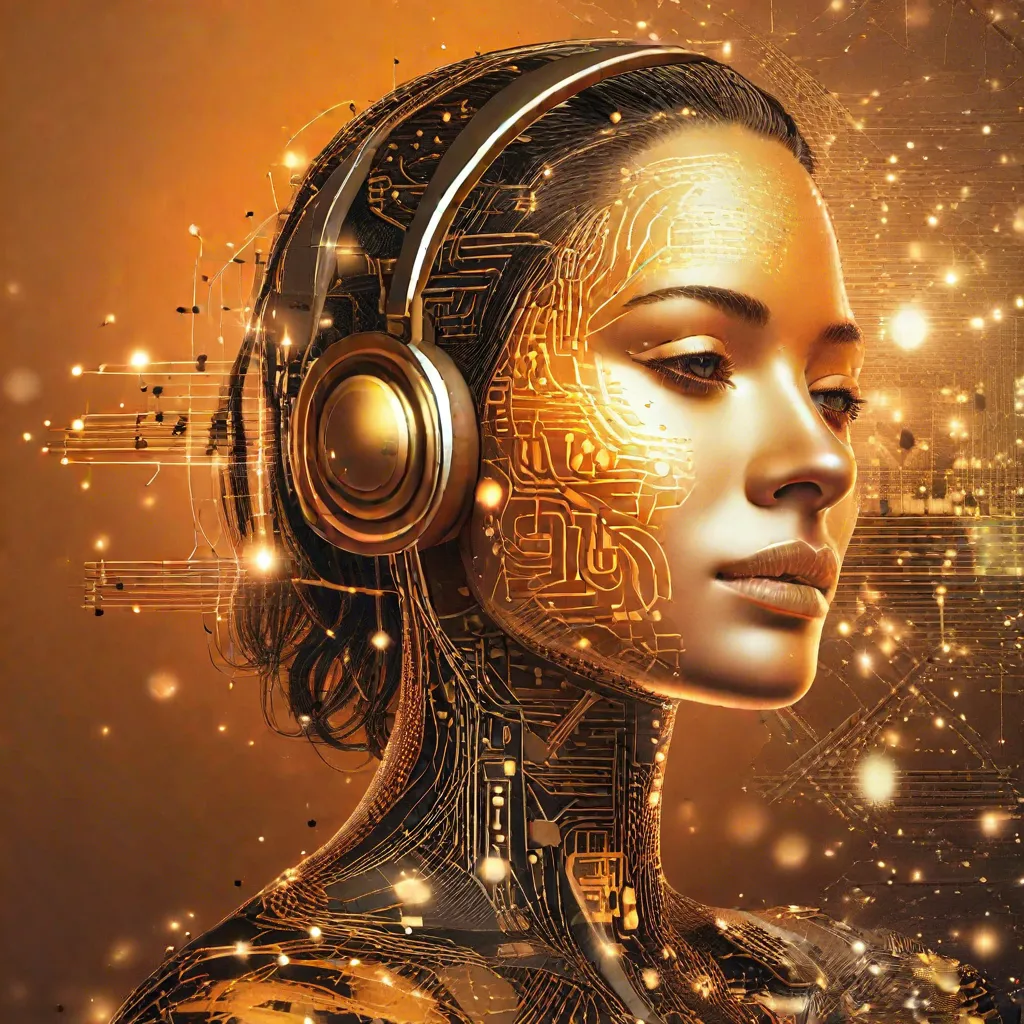
\includegraphics[width=.8\columnwidth]{ai_w_headphones}%
        \end{figure}
    \end{columns}
\end{frame}